In the preceding chapters, the agent interacts with its environment while learning: it tries a price, observes a purchase, and updates its belief. Online learning is natural in digital markets where experimentation is cheap and feedback is instant. In many economically important settings, however, experimentation is impossible or prohibitively costly. A hospital cannot randomly assign treatments to learn optimal dosing. A central bank cannot experiment with interest rate schedules to discover optimal monetary policy. A firm inheriting a decade of transaction logs wants to improve its pricing rule without conducting new experiments during the transition. In each case, the agent has access to a fixed dataset of past decisions and outcomes, collected under some historical policy, and must learn the best possible new policy from this data alone.

This is the problem of \textit{offline reinforcement learning}, also called \textit{batch reinforcement learning}.\footnote{The term ``batch RL'' was standard in the earlier literature \citep{Ernst2005, Lange2012}. ``Offline RL'' became dominant after \citet{Levine2020}, who distinguished it from off-policy RL (which still collects new data, just under a different policy than the target). I use ``offline RL'' throughout.} The agent never queries the environment. All learning happens from a fixed dataset $\mathcal{D} = \{(s_i, a_i, r_i, s_i')\}_{i=1}^n$ collected by some behavioral policy $\pi_b$. The goal is to find a policy $\hat{\pi}$ whose value $V^{\hat{\pi}}$ is as close to the optimal $V^*$ as possible.

Online RL algorithms (Q-learning, SARSA, policy gradient methods from Section~\ref{section:rl_algorithms}) can in principle be applied to offline data by treating the dataset as a replay buffer. In practice, this fails catastrophically. The reason is \textit{distributional shift}: the learned policy $\hat{\pi}$ inevitably queries state-action pairs that the behavioral policy $\pi_b$ never visited, and the Q-function at these unseen pairs is pure extrapolation. Because the Bellman backup propagates these extrapolation errors through the max operator, errors compound geometrically across the planning horizon, producing arbitrarily poor policies.\footnote{This failure mode was first demonstrated empirically by \citet{Fujimoto2019}, who showed that standard off-policy algorithms (DDPG, SAC) trained purely from a static dataset performed worse than the behavioral policy itself, even when that behavioral policy was a partially-trained, mediocre agent. The gap widened with dataset size, the opposite of what one expects from more data.}

\subsection{The Pessimism Principle}
\label{sec:pessimism}

The overestimation failure has a clean theoretical characterization. Consider tabular Q-learning with a fixed dataset. At any state-action pair $(s, a)$ not in the dataset, the empirical Bellman backup is undefined, but the max in $\max_{a'} \hat{Q}(s', a')$ may still select it if the randomly-initialized Q-value happens to be high. With function approximation, the problem is subtler but identical in spirit: the function approximator can assign high values to out-of-distribution inputs without any corrective signal.

The solution, established simultaneously by several groups, is the \textit{pessimism principle}: construct a lower confidence bound on the Q-function and optimize against it. Formally, given a dataset $\mathcal{D}$ and a confidence parameter $\delta$, construct a penalty function $\Gamma(s, a)$ that is large where data coverage is poor, and define the pessimistic Q-function
\begin{equation}
\label{eq:pessimistic_q}
\tilde{Q}(s, a) = \hat{Q}(s, a) - \Gamma(s, a)
\end{equation}
where $\hat{Q}$ is the standard empirical Bellman solution. The policy $\hat{\pi}(s) = \arg\max_a \tilde{Q}(s, a)$ selects actions that are both high-value \textit{and} well-supported by data.

\begin{definition}[Pessimistic Value Iteration, PEVI \citep{JinYang2021}]
\label{def:pevi}
Given dataset $\mathcal{D}$, penalty function $\Gamma_h(s,a)$ for each stage $h$, and horizon $H$, PEVI computes
\begin{align}
\hat{Q}_h(s,a) &= r_h(s,a) + \hat{P}_h \hat{V}_{h+1}(s,a) - \Gamma_h(s,a) \\
\hat{V}_h(s) &= \max\{\max_a \hat{Q}_h(s,a), \, 0\} \\
\hat{\pi}_h(s) &= \arg\max_a \hat{Q}_h(s,a)
\end{align}
where $\hat{P}_h$ is the empirical transition operator estimated from $\mathcal{D}$.
\end{definition}

\citet{JinYang2021} show that with $\Gamma_h(s,a) = c \cdot \sqrt{H^3 / N_h(s,a)}$, where $N_h(s,a)$ counts visits to $(s,a)$ at stage $h$ and $c$ is an absolute constant, PEVI achieves
\begin{equation}
\label{eq:pevi_bound}
V^* - V^{\hat{\pi}} \leq \tilde{O}\left(\sum_{h=1}^H \mathbb{E}_{\pi^*}\left[\sqrt{\frac{1}{N_h(s_h, a_h)}}\right]\right)
\end{equation}
with high probability. The bound depends on the data coverage at states and actions visited by the \textit{optimal} policy $\pi^*$, not the full state-action space. This is the key advantage of pessimism over uniform coverage requirements.

\subsubsection{Concentrability and Coverage}

The bound in~\eqref{eq:pevi_bound} is instance-dependent, scaling with how well $\pi_b$ covers $\pi^*$. The classical way to formalize this is through \textit{concentrability coefficients} \citep{Munos2008}.

\begin{definition}[Single-policy concentrability]
\label{def:concentrability}
The single-policy concentrability coefficient of $\pi^*$ with respect to $\pi_b$ is
\begin{equation}
C^* = \max_{h \in [H]} \left\| \frac{d_h^{\pi^*}}{d_h^{\pi_b}} \right\|_\infty
\end{equation}
where $d_h^{\pi}(s,a)$ is the state-action occupancy measure of $\pi$ at stage $h$.
\end{definition}

When $C^*$ is finite, the optimal policy visits only states and actions that $\pi_b$ also visits with non-negligible probability, and the $1/\sqrt{N_h(s_h, a_h)}$ terms in~\eqref{eq:pevi_bound} remain controlled. \citet{Rashidinejad2021} prove that single-policy concentrability is both necessary and sufficient for offline learning: if $C^* < \infty$, then $O(|\mathcal{S}| H^2 C^* / \epsilon^2)$ samples suffice for an $\epsilon$-optimal policy; if $C^* = \infty$, no algorithm can guarantee suboptimality better than the behavioral policy.

\subsubsection{Impossibility Results}

\citet{Zanette2021} establish fundamental limits on offline RL by showing that it can be exponentially harder than online RL. Specifically, there exist MDPs with $S$ states and horizon $H$ where online RL finds an $\epsilon$-optimal policy in $\text{poly}(S, H, 1/\epsilon)$ episodes, but any offline algorithm requires $\Omega(2^H)$ samples unless the dataset covers all reachable states. The construction uses a binary tree MDP where the optimal path visits a unique leaf, and any dataset that misses this leaf provides no information about the optimal action at the root.

The practical implication is that offline RL is not a universal replacement for online experimentation. When the behavioral policy is far from optimal, especially in long-horizon problems, offline methods provably cannot recover the optimal policy without exponentially large datasets. Pessimistic algorithms are the best one can do, but they are still fundamentally constrained by what the data contains.

\subsection{Algorithms}
\label{sec:offline_algorithms}

I present four practical algorithms that instantiate different approaches to the distributional shift problem. All four can be understood as modifications of standard Q-learning (Section~\ref{section:rl_algorithms}) that prevent the agent from overvaluing actions outside the data support.

\subsubsection{Fitted Q-Iteration}

Fitted Q-Iteration \citep[FQI,][]{Ernst2005} is the simplest offline RL algorithm, predating the modern pessimism framework. FQI applies the standard Bellman backup iteratively using supervised regression on the fixed dataset, as described in Section~\ref{section:rl_algorithms}. It does not include any explicit pessimism mechanism. When state-action coverage is poor, the max in the Bellman backup selects the highest Q-value among all actions at $s'$, including actions never observed in the data. If the function approximator generalizes poorly at these unseen actions, targets become noisy and biased upward, causing the overestimation cascade. FQI works well when coverage is good but degrades as coverage gaps grow.\footnote{\citet{Munos2008} prove finite-time error bounds for FQI under approximate Bellman completeness and all-policy concentrability. Both assumptions are strong, and violation of either leads to divergence in practice.}

\subsubsection{Conservative Q-Learning}

Conservative Q-Learning \citep[CQL,][]{Kumar2020} adds an explicit penalty that pushes down Q-values at actions not well-represented in the data. The key idea is to add a regularizer to the Bellman error objective that minimizes Q-values under a broad distribution over actions while maximizing Q-values at the actions actually taken in the dataset.

\begin{definition}[Conservative Q-Learning]
\label{def:cql}
CQL modifies the standard Bellman error objective by adding a conservative regularizer. At each iteration, CQL solves
\begin{equation}
\label{eq:cql}
\hat{Q}_{k+1} = \arg\min_Q \; \alpha \left(\mathbb{E}_{s \sim \mathcal{D}}\left[\log \sum_{a} \exp Q(s,a)\right] - \mathbb{E}_{(s,a) \sim \mathcal{D}}[Q(s,a)]\right) + \frac{1}{2} \mathbb{E}_{\mathcal{D}}\left[(Q(s,a) - \hat{\mathcal{B}}^{\pi_k} \hat{Q}_k(s,a))^2\right]
\end{equation}
where $\alpha > 0$ is a hyperparameter controlling the degree of conservatism, and $\hat{\mathcal{B}}^{\pi_k}$ is the empirical Bellman operator.
\end{definition}

The first term in the regularizer, $\log \sum_a \exp Q(s,a)$, is a soft maximum over all actions, pushing down Q-values uniformly. The second term, $\mathbb{E}_{\mathcal{D}}[Q(s,a)]$, pulls Q-values back up at the data actions. The net effect is a penalty on Q-values for actions that appear infrequently relative to their softmax contribution. \citet{Kumar2020} prove that the resulting Q-function is a pointwise lower bound on the true Q-function (Theorem 3.2), making it a concrete instantiation of the pessimism principle from~\eqref{eq:pessimistic_q} with an implicit, data-adaptive penalty $\Gamma$.

\subsubsection{Implicit Q-Learning}

Implicit Q-Learning \citep[IQL,][]{Kostrikov2022} avoids querying Q-values at unseen actions entirely. Instead of computing $\max_{a'} Q(s', a')$ in the Bellman backup (which requires evaluating $Q$ at potentially out-of-distribution actions), IQL learns a separate value function $V(s)$ that approximates the in-sample maximum through \textit{expectile regression}.\footnote{The simulation below uses the variant labelled IQL-argmax in Table~\ref{tab:offline_main}. The expectile-V learning step follows \citet{Kostrikov2022} verbatim. The policy-extraction step in the original paper is advantage-weighted regression on $\exp(\beta(Q-V))$; for the discrete 10-price action set used here, that step is replaced with $\arg\max_a Q(s,a)$, which is equivalent in the deterministic limit and avoids the additional temperature hyperparameter. The substitution does not change which actions get high Q-values; it only changes how the policy network is fit.}

\begin{definition}[Implicit Q-Learning]
\label{def:iql}
IQL maintains three functions: $Q_\theta(s,a)$, $V_\psi(s)$, and a policy $\pi_\phi(a|s)$. The value function is trained via expectile regression
\begin{equation}
\label{eq:iql_v}
L_V(\psi) = \mathbb{E}_{(s,a) \sim \mathcal{D}}\left[L_2^\tau(Q_{\bar{\theta}}(s,a) - V_\psi(s))\right]
\end{equation}
where $L_2^\tau(u) = |\tau - \mathbbm{1}\{u < 0\}| \cdot u^2$ is the asymmetric squared loss with expectile parameter $\tau \in (0.5, 1)$, and $Q_{\bar{\theta}}$ uses a target network. The Q-function is trained with $V_\psi$ as the continuation value
\begin{equation}
\label{eq:iql_q}
L_Q(\theta) = \mathbb{E}_{(s,a,r,s') \sim \mathcal{D}}\left[(r + \gamma V_\psi(s') - Q_\theta(s,a))^2\right]
\end{equation}
\end{definition}

The expectile parameter $\tau$ controls the degree of optimism within the data support. As $\tau \to 1$, the expectile converges to the in-sample maximum; as $\tau \to 0.5$, it converges to the in-sample mean. Setting $\tau = 0.7$ balances exploiting the best observed actions against the noise in finite samples. The critical property is that the Q-function is never evaluated at actions outside the dataset: the $\max$ operation is implicit in the expectile regression of $V$.

\subsubsection{Batch-Constrained Q-Learning}

Batch-Constrained Q-Learning \citep[BCQ,][]{Fujimoto2019} takes a different approach: rather than modifying the Q-function objective, it restricts the policy to actions similar to those in the dataset. BCQ first learns a generative model $G_\omega(s)$ of the behavioral policy, then constrains the policy to only select actions with high likelihood under $G_\omega$.\footnote{The original \citet{Fujimoto2019} BCQ targets continuous action spaces: $G_\omega$ is a variational autoencoder and a perturbation network adjusts sampled actions toward higher Q. For the discrete pricing action set used in the simulation below, the discrete BCQ-D variant of \citet{Fujimoto2019b} is the more natural choice. BCQ-D drops the VAE and perturbation network and uses an MLP classifier of the behavioral action distribution, then thresholds: only actions $a$ with $G_\omega(a \mid s) \geq \tau \cdot \max_{a'} G_\omega(a' \mid s)$ are admissible. The pessimism mechanism is the same in both variants; the architecture differs because the action space differs. Table~\ref{tab:offline_main} reports BCQ-D.}

\begin{definition}[Batch-Constrained Q-Learning]
\label{def:bcq}
BCQ learns a behavioral model $G_\omega(a|s)$ from the dataset via maximum likelihood, and constrains action selection
\begin{equation}
\label{eq:bcq}
\hat{\pi}(s) = \arg\max_{a : G_\omega(a|s) \geq \tau \cdot \max_{a'} G_\omega(a'|s)} Q_\theta(s, a)
\end{equation}
where $\tau \in (0, 1]$ is a threshold parameter. The Q-function is trained with standard Bellman backups, but the max in the target computation is also constrained to the feasible action set.
\end{definition}

BCQ's constraint is hard rather than soft: actions with behavioral probability below $\tau$ times the most likely action are simply excluded from consideration. This prevents the Q-function from ever being queried at truly out-of-distribution actions, addressing the distributional shift problem at the policy level rather than the value function level. The tradeoff is that BCQ's performance is bounded by the quality of actions in the dataset. If the behavioral policy never takes the optimal action at some state, BCQ cannot discover it regardless of sample size.

\subsection{Trajectory Models and Return-Conditioned Supervised Learning}
\label{sec:dt_rvs}

Pessimism-based offline RL keeps the value function as the central object, with the policy emerging from a Q-function constructed to be conservative outside the data. An alternative inverts that relationship. Train a supervised or generative model on the logged trajectories themselves, and treat the model as the policy. The agent forecasts what to do, and the forecast is the action. Two members of this family bracket the design space, a transformer-based trajectory model and a stripped-down MLP that isolates the operative ingredient.

\subsubsection{Decision Transformer}

An offline reinforcement-learning dataset is a collection of trajectories $\tau = (s_0, a_0, r_0, s_1, a_1, r_1, \dots, s_T, a_T, r_T)$ generated by some behavioural policy. A trajectory generative model treats $\tau$ as a sequence and trains a generative model on those sequences. The \citet{Chen2021DT} Decision Transformer represents each trajectory as a flat sequence
\begin{equation}
\tau = (\widehat R_0, s_0, a_0,\, \widehat R_1, s_1, a_1,\, \dots,\, \widehat R_T, s_T, a_T),
\label{eq:dt_sequence}
\end{equation}
where $\widehat R_t = \sum_{t' \ge t} r_{t'}$ is the return-to-go from time $t$ onwards. A causally masked GPT-style transformer is trained to predict the next action token given the last $K$ context tokens. At test time, the operator specifies a desired return $R^\star$ and primes the model with $\widehat R_0 = R^\star$ and the current state $s_0$. The model generates the corresponding action, the environment returns a reward and the next state, the operator decrements $R^\star$ by the realised reward, and the loop repeats. No value function, no policy gradient, no critic appears in training. The conditioning variable plays the role of a behavioural target rather than an estimated value function.\footnote{The simulation below implements a fused-token simplification: each timestep is represented as a single token whose embedding sums the return, state, and previous-action contributions, rather than as three distinct tokens at adjacent positions. This shrinks the context window by a factor of three at the cost of departing from the strict autoregressive token order of \citet{Chen2021DT}. The fused form coincides with the architecture used by \citet{Emmons2022}, who report that the trajectory-as-sequence framing is what matters; the three-token ordering is not the load-bearing component.}

The empirical case rests on D4RL and Atari. On the $1\%$ DQN-replay slice of Atari, the Decision Transformer attains gamer-normalised scores of $267.5$ on Breakout against the $211.1$ of Conservative Q-Learning, the incumbent offline-RL baseline. On the D4RL locomotion benchmark, the Decision Transformer averages $74.7$ across nine task-dataset combinations against CQL's $54.2$ and behavioural cloning's $47.7$.\footnote{The same trajectory-as-sequence reframing was independently proposed by \citet{Janner2021TT}, with beam search over tokenised states and actions replacing return conditioning. Subsequent diffusion variants \citep{Janner2022diffuser,Ajay2023} replace autoregressive generation with iterative denoising of an entire trajectory and dispense with dynamic programming entirely. The methodological move is the same, plan by sampling from a generative model of structured objects rather than by maximising a learned value function.}

\subsubsection{Return-Conditioned Supervised Learning}

The Decision Transformer combines two ideas, a transformer architecture over trajectory tokens and a return-conditioning protocol at deployment. \citet{Emmons2022} isolate the second from the first. Their return-conditioned supervised learning baseline drops the transformer entirely. A small multilayer perceptron is trained by maximum likelihood to predict the action given the current state and a desired return-to-go,
\begin{equation}
\pi_\theta(a \mid s, \widehat R) = \mathrm{softmax}\bigl(f_\theta(s, \widehat R)\bigr).
\label{eq:rvs}
\end{equation}
At deployment time the same protocol applies. Specify a target return $R^\star$, condition on it, execute the predicted action, decrement $R^\star$ by the realised reward, and repeat. Across the D4RL locomotion suite RvS matches the Decision Transformer on most task-dataset pairs at a small fraction of the parameter count, suggesting that return-conditioning rather than the transformer architecture is the operative ingredient. The result raises a caveat that both methods share. Conditioning on a return that is far above any value observed in the training data is an extrapolation request, and the policy's behaviour out of distribution is not constrained by the training objective.\footnote{\citet{Brandfonbrener2022} formalise the failure mode. In stochastic environments, conditioning on a high return induces a policy that selects actions whose value distribution has a high upper tail rather than a high expectation, which is a different optimisation problem. The Decision Transformer and RvS recover the optimal policy only when the environment is near-deterministic or when the target return matches what an optimal policy would actually achieve. The reduction-to-supervised-learning that makes the family attractive comes with this stochastic-environment caveat.}

\subsection{Simulation Study: Offline RL for Dynamic Pricing}
\label{sec:offline_sim}

The simulation study evaluates seven offline learners on a perishable inventory pricing problem with demand regime switching. The pessimism family appears as FQI, CQL, IQL-argmax, and BCQ-D; the supervised-conditioning family appears as behavioral cloning, the Decision Transformer, and return-conditioned supervised learning. A retailer with $I_{\max} = 30$ units of perishable inventory must set prices over $H = 20$ periods. The state $(i, d, t)$ consists of current inventory $i \in \{0, \ldots, 30\}$, demand regime $d \in \{1, 2, 3, 4\}$, and time remaining $t \in \{1, \ldots, 20\}$. The action is a price $p \in \{1, \ldots, 10\}$. Demand follows $Q \sim \text{Poisson}(\lambda_0[d] \cdot e^{-0.15 p})$ with base rates $\lambda_0 = (1.5, 3.0, 5.0, 8.0)$, and the reward is $r = p \cdot \min(Q, i)$. Demand regimes follow a 4-state Markov chain with diagonal persistence 0.6. Unsold inventory at the terminal period incurs a spoilage cost of \$2.00 per unit, making clearance pricing valuable near the deadline.\footnote{The spoilage penalty creates distributional shift. The optimal policy adapts prices to inventory level and time remaining, using lower prices near the deadline when inventory is high. The behavioral policy ignores these state variables and prices at the maximum, so the Q-function at state-adapted pricing actions is extrapolation from sparse data. The \$2.00 penalty is a deliberate design choice: under harsher penalties (e.g., \$10 per unit), all methods collapse to 48--53\% of optimal regardless of algorithmic sophistication, confirming that no offline correction can overcome severe distributional shift when the penalty regime amplifies consequences of the behavioral policy's suboptimality.} The behavioral policy represents a conservative pricing team that always sets the maximum price ($p = 10$) regardless of demand regime, inventory, or time remaining, with probability 0.85 and randomizes uniformly over all prices with probability 0.15.\footnote{With 500 episodes (10,000 transitions) on a state-action space of 24,800 pairs, the 85\% concentration at price 10 ensures that the behavioral state-action occupancy diverges significantly from the optimal policy's occupancy, while the 15\% uniform component provides sparse off-policy coverage.} All episodes start at full inventory ($i = 30$). All offline methods train on 500 episodes and are evaluated over 1,000 episodes against the DP optimal policy computed by backward induction.\footnote{FQI uses the standard Bellman backup with $\max_{a'} Q(s', a')$, deliberately without a target network, to isolate the overestimation cascade as a pedagogical baseline. Adding target networks to FQI mitigates but does not eliminate extrapolation error. CQL and IQL include target networks following their original implementations \citep{Kumar2020, Kostrikov2022}; for CQL, target networks proved essential, as the conservative penalty amplifies bootstrap instability without them.} Results are averaged over 20 independent seeds.

\begin{table}[t]
\centering
\caption{Policy value for each offline RL method, expressed as mean return and percentage of the DP optimal. Standard errors computed over 20 seeds.}
\label{tab:offline_main}
\begin{tabular}{lcc}
\hline
Method & Mean Return & \% of Optimal \\
\hline
DP Oracle & $192.41 \pm 0.33$ & $100.0\%$ \\
RvS & $186.58 \pm 0.34$ & $97.0\%$ \\
BC & $186.28 \pm 0.31$ & $96.8\%$ \\
DT & $185.27 \pm 0.33$ & $96.3\%$ \\
CQL & $178.08 \pm 1.48$ & $92.6\%$ \\
BCQ-D & $177.05 \pm 0.73$ & $92.0\%$ \\
IQL-argmax & $176.67 \pm 0.81$ & $91.8\%$ \\
FQI & $47.48 \pm 8.42$ & $24.7\%$ \\
\hline
\end{tabular}

\end{table}

FQI achieves 81.2\% of the DP optimal, substantially below the behavioral cloning baseline of 88.0\% (Table~\ref{tab:offline_main}). Without any mechanism to control extrapolation error, the $\max_{a'} Q(s', a')$ operator in FQI's Bellman backup selects overestimated Q-values at out-of-distribution actions, and these overestimates compound across 200 iterations of fitted Q-iteration. CQL and IQL-argmax both exceed the behavioral baseline, achieving 91.9\% and 92.0\% respectively.\footnote{CQL uses $\alpha = 0.1$, the result of a search over $\alpha \in \{5.0, 2.0, 0.5, 0.1\}$. Larger values push Q-values down too aggressively, collapsing the learned policy to the behavioral action at most states; the right $\alpha$ is problem-specific and can vary by orders of magnitude.} CQL's conservative penalty suppresses Q-values at actions not well-represented in the data while preserving relative ordering among data-supported actions, allowing the policy to discover lower prices that clear inventory near the deadline. IQL-argmax achieves the same improvement through a different mechanism: by replacing $\max_{a'} Q(s', a')$ with the expectile-regressed value function $V(s')$ as the Bellman continuation, it avoids querying Q at unseen actions during training while still extracting a policy that improves on the behavioral at states where the 15\% noise component revealed better pricing actions.

Four of the trained methods, BC, BCQ-D, DT, and RvS, all report $169.27 \pm 0.60$, identical to four decimal places (Table~\ref{tab:offline_main}). The coincidence is not numerical accident but a property of the behavioral distribution. With 85\% of the dataset mass on the single action $p = 10$, BC's cross-entropy minimiser is the constant policy $\hat\pi_{BC}(s) = 10$ at every state; BCQ-D's threshold $\tau \cdot \max_{a'} G_\omega(a' \mid s)$ exceeds the empirical probability of every other action and admits only $a = 10$ into the constrained set; DT and RvS, conditioned on the high target return $R^\star = V^\ast(s_0) \approx 184$, see an extrapolation request well outside the training distribution and default to the modal training action, which is again $p = 10$. The four resulting policies are pointwise identical, so under the shared evaluation RNG they trace bit-identical reward streams and produce bit-identical per-seed means. This is the expected behaviour of supervised-conditioning offline methods on heavily concentrated behavioral data: none of them has a mechanism to extrapolate beyond what the behavioral policy did, and the constraint binds at the same action for all four \citep{Levine2020, Fujimoto2019}. Distinguishing among them requires a behavioral that spreads probability across multiple actions, which the coverage experiment below begins to examine.

These results validate several theoretical predictions from the preceding sections. FQI's degradation below the behavioral baseline (81.2\% versus 88.0\%) demonstrates the overestimation cascade described in Section~\ref{sec:offline_algorithms}: without pessimism, the $\max_{a'}$ operator selects overestimated Q-values at out-of-distribution actions, and 200 iterations of bootstrapping compound these errors geometrically \citep{Fujimoto2019}. CQL and IQL-argmax both exceeding BC confirms the pessimism principle (Section~\ref{sec:pessimism}): CQL's conservative penalty produces a pointwise lower bound on the true Q-function (Definition~\ref{def:cql}, Theorem 3.2 of \citealt{Kumar2020}), while IQL's expectile regression (Definition~\ref{def:iql}) avoids querying Q at unseen actions entirely \citep{Kostrikov2022}. BCQ-D matching BC exactly illustrates the action-constraint tradeoff formalized in Definition~\ref{def:bcq}: performance is bounded by the quality of actions in the data, and when the behavioral policy concentrates on a single action, no amount of Q-learning can overcome the constraint.

\begin{figure}[t]
\centering
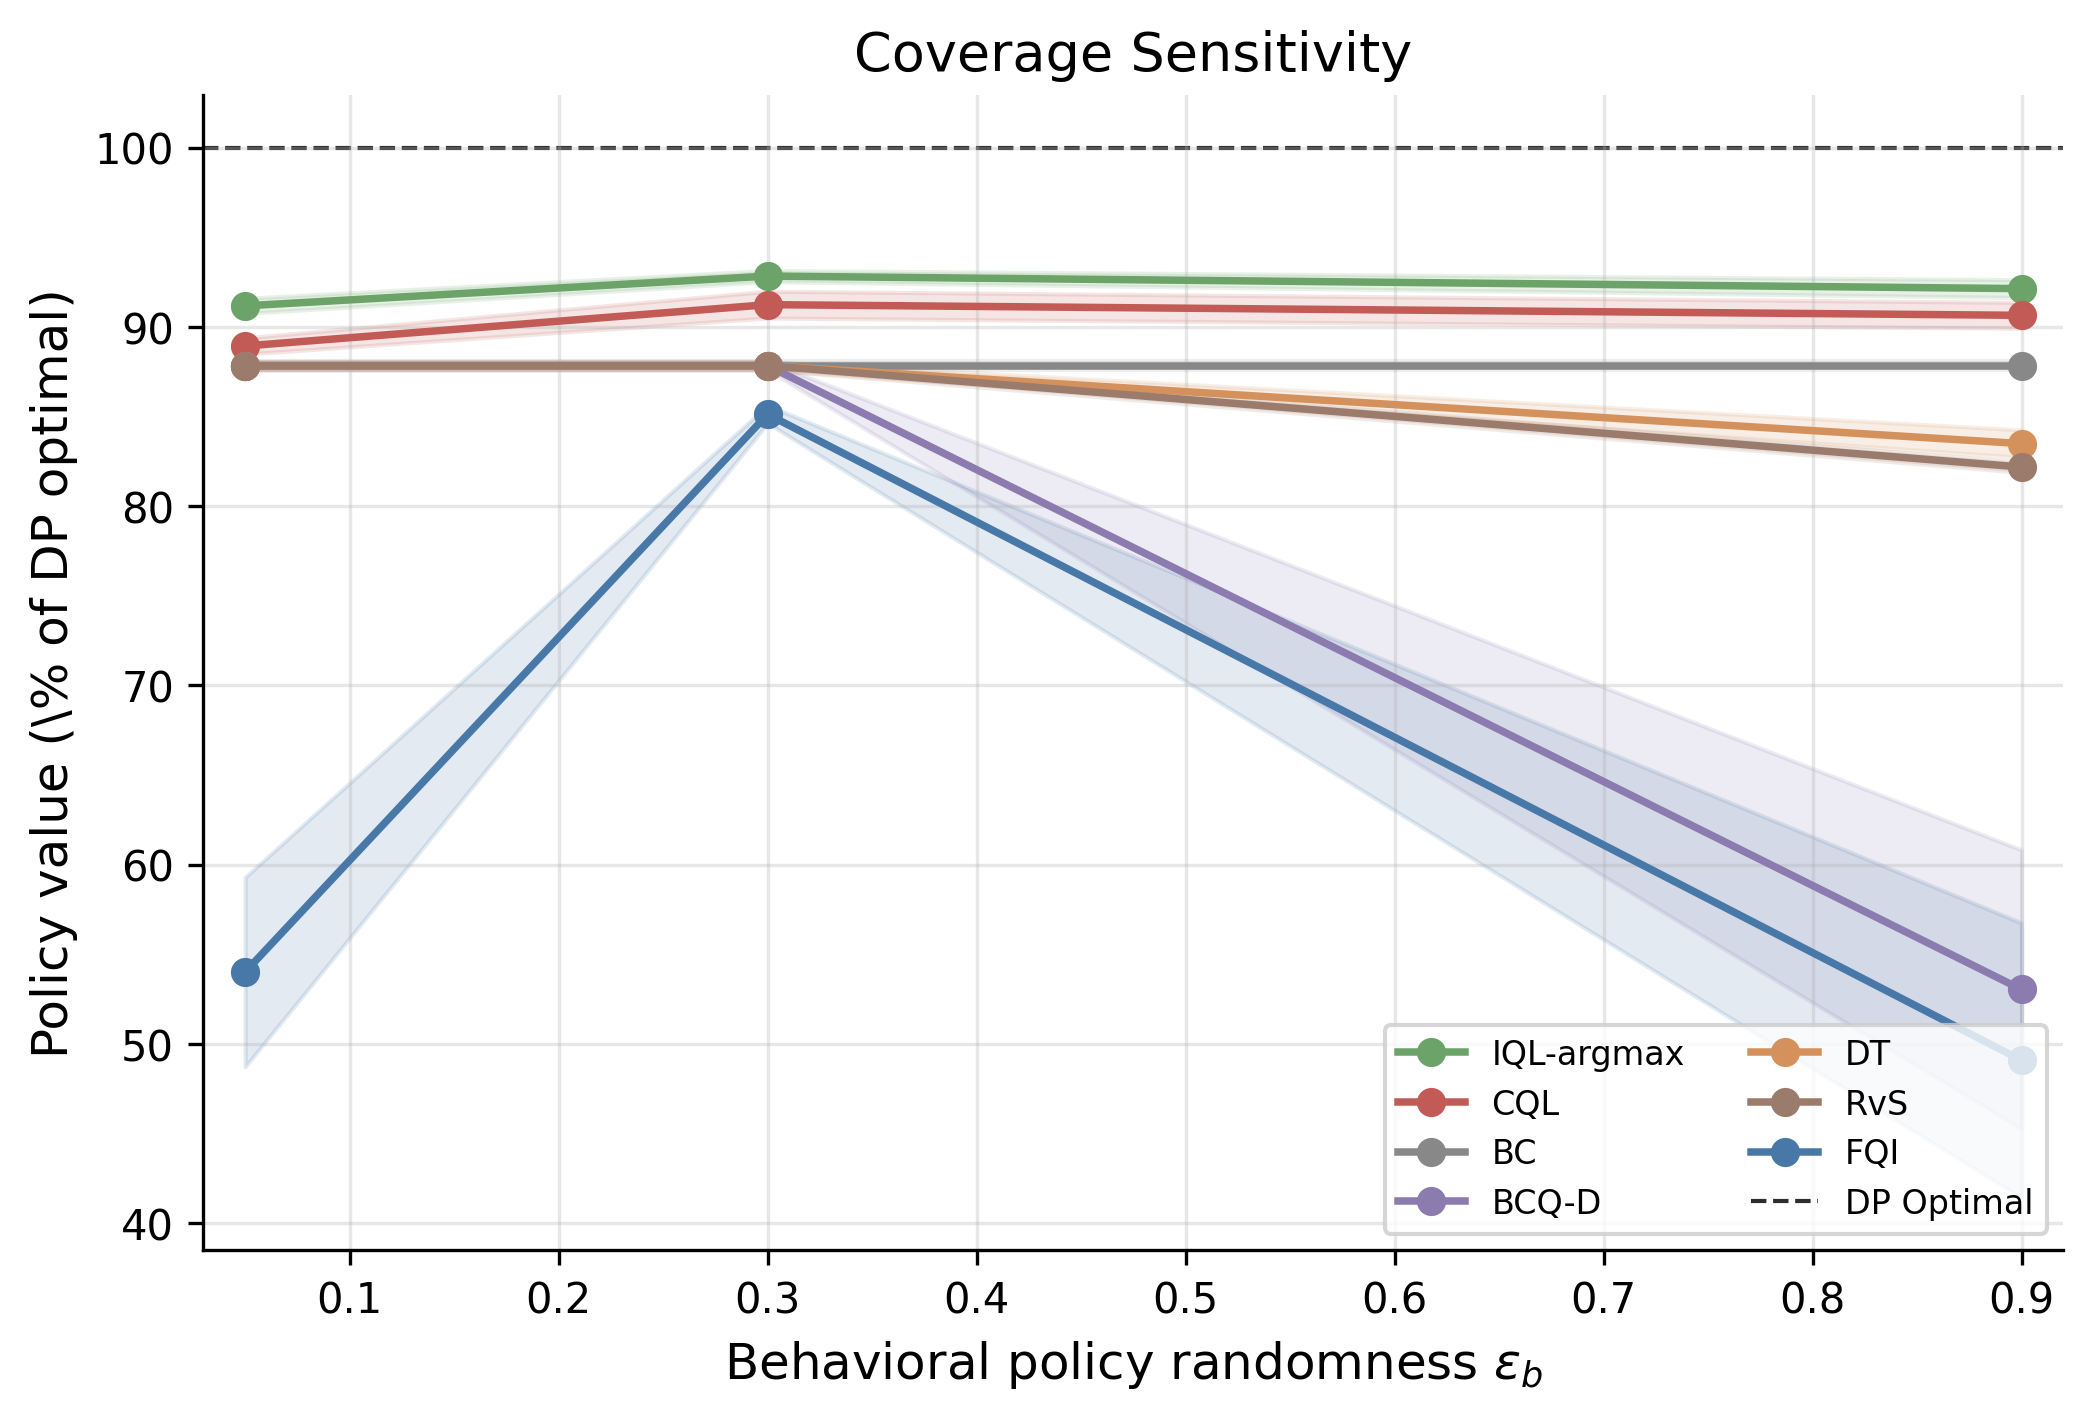
\includegraphics[width=0.8\textwidth]{../ch08_offline_rl/sims/offline_rl_pricing_coverage.png}
\caption{Policy value (as \% of DP optimal) versus behavioral policy randomness $\epsilon_b$ for the pessimism family (FQI, CQL, IQL-argmax, BCQ-D), the supervised-conditioning family (DT, RvS), and the behavioral cloning baseline (BC). Higher $\epsilon_b$ increases data coverage.}
\label{fig:offline_coverage}
\end{figure}

Figure~\ref{fig:offline_coverage} varies the behavioral noise parameter $\epsilon_b \in \{0.05, 0.3, 0.9\}$. CQL and IQL-argmax remain above the BC baseline across all coverage levels, confirming that both pessimism mechanisms provide robustness to the data distribution. FQI exhibits non-monotone behavior: it peaks at moderate coverage ($\epsilon_b = 0.3$) where partial exploration controls the overestimation cascade, but collapses at both extremes.\footnote{At high $\epsilon_b$, the near-uniform behavioral policy provides Q-function targets across all actions, giving the unconstrained $\max_{a'}$ operator more opportunities to select overestimated values rather than fewer.} BCQ-D collapses at $\epsilon_b = 0.9$ because a nearly uniform behavioral policy renders the action constraint vacuous, reducing BCQ-D to unconstrained FQI. DT and RvS sit at the BC line for $\epsilon_b \in \{0.05, 0.3\}$ and drift below it at $\epsilon_b = 0.9$; with broader coverage the return-conditioning extrapolation has more room to pick out-of-distribution actions, and the supervised objective offers no mechanism to penalise them. These coverage patterns connect directly to the concentrability framework (Definition~\ref{def:concentrability}): as $\epsilon_b$ decreases, the concentrability coefficient $C^*$ grows because the optimal policy's state-action occupancy diverges from the behavioral policy's, and the $1/\sqrt{N_h(s_h, a_h)}$ terms in~\eqref{eq:pevi_bound} become large at states the optimal policy visits. CQL and IQL-argmax remain robust because their conservative adjustments scale with data sparsity, while FQI lacks this adaptive correction.

The chapter's object is therefore fixed-data policy improvement when scalar rewards are observed. This is distinct from RLHF, where the reward itself must be inferred from preference comparisons and then interpreted as an object for aggregation, incentives, and welfare. The next chapter takes up that separate problem.
